\section{Work Efficiency Metric} \label{sec:metric}

    In this section we define work efficiency, a metric for comparing different optimized versions of a program when executing with
    different inputs. We define it as the ratio between the amount of \textit{work}, $\Delta W$, performed during a period of time, $\Delta
    t$.

    \[
       P = \nicefrac{\Delta W}{\Delta t}
    \]

    The main challenge is to precisely define what represents \textit{work}. We define the work done by a program on an input to be the
    time taken by the unoptimized program to process that input. We estimate the runtime of each instruction type and then work is the sum
    of the runtime for each instruction type multiplied by its dynamic count.
    
    \[ \Delta W = \sum_i w_i.n_i \]
    
    Where $i$ is the instruction type, $w_i$ is the estimated runtime for instruction type $i$, and $n_i$ is the number of observed
    executions of instruction type $i$.

    Similarly to previous work~\citep{giusto01,powell09,brandolese11}, the coefficients, $w_i$, are found by linear regression. We create
    one data point for the regressor for a set of program and input pairs. The programs are given in Table~\ref{tab:kdatasets:training},
    and each has 1,000 inputs. The response variable is the runtime of the unoptimized program as it processes the input. To ensure
    statistically sound results, the runtime is measured by repeated execution until the 99\% confidence interval is no larger than 1\% of
    the mean. The explanatory variables are the dynamic instruction counts for each program and input. They are recorded by a separate,
    instrumented run of the program on the input.

    Figure~\ref{fig:cost-model} shows the correlation of the model with runtime on instances of test benchmarks. The correlation
    coefficient is \FIXME{XXX}, and the mean absolute percentage error (MAPE) is \FIXME{XXX}. Figure~\ref{fig:motivation-work-efficiency}
    shows a similar plot to Figure~\FIXME{\ref{fig:???}}, of work efficiency versus speedup for 500 different binaries of \texttt{susan\_c}. Here the new metric correlates much better than either performance or IPC.

    \begin{figure}[t]
        \centering
        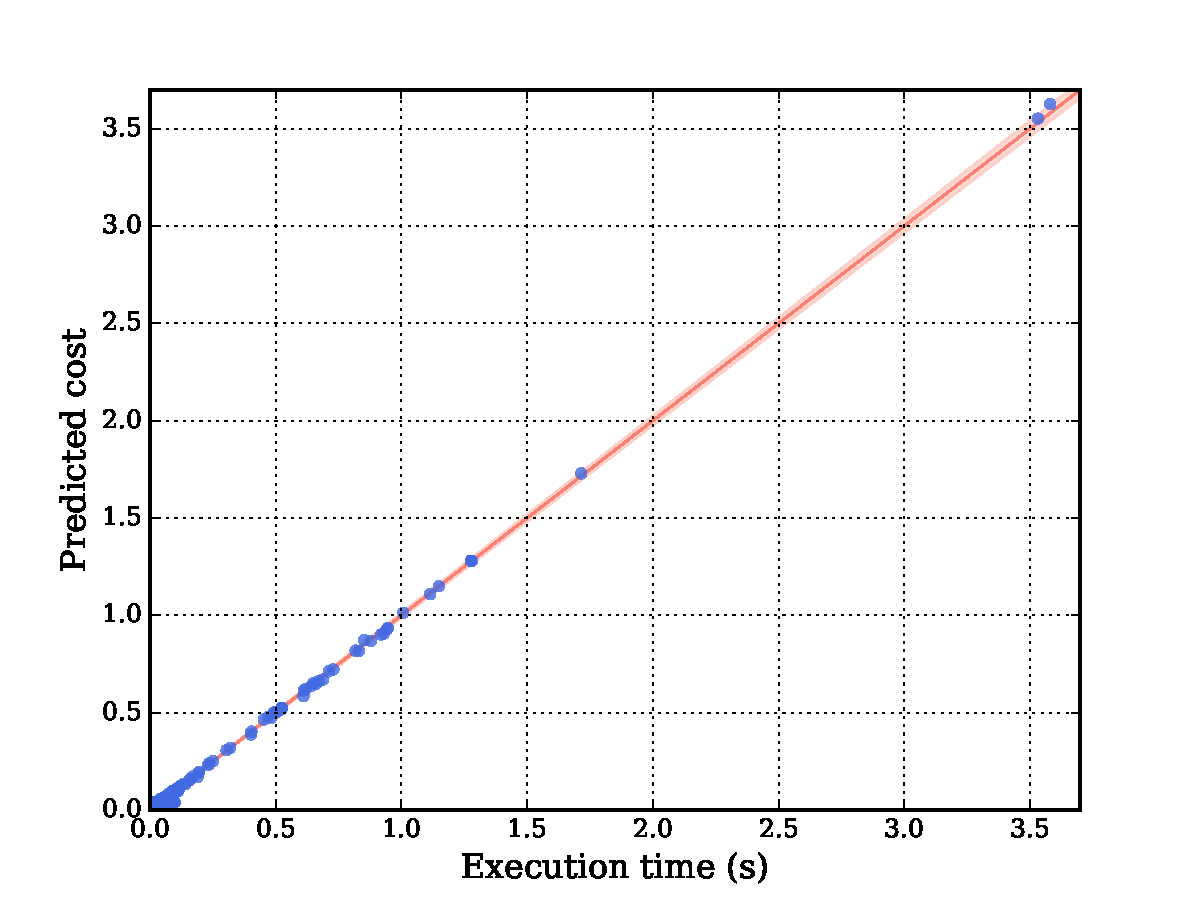
\includegraphics[width=0.6\linewidth]{figs/cost-model.pdf}
        \caption{
            Linear model for work metric fitted from empirical data.
            \red{zw: bigger font size.}
        }
        \label{fig:cost-model}
    \end{figure}

    \begin{figure}[t]
        \centering
        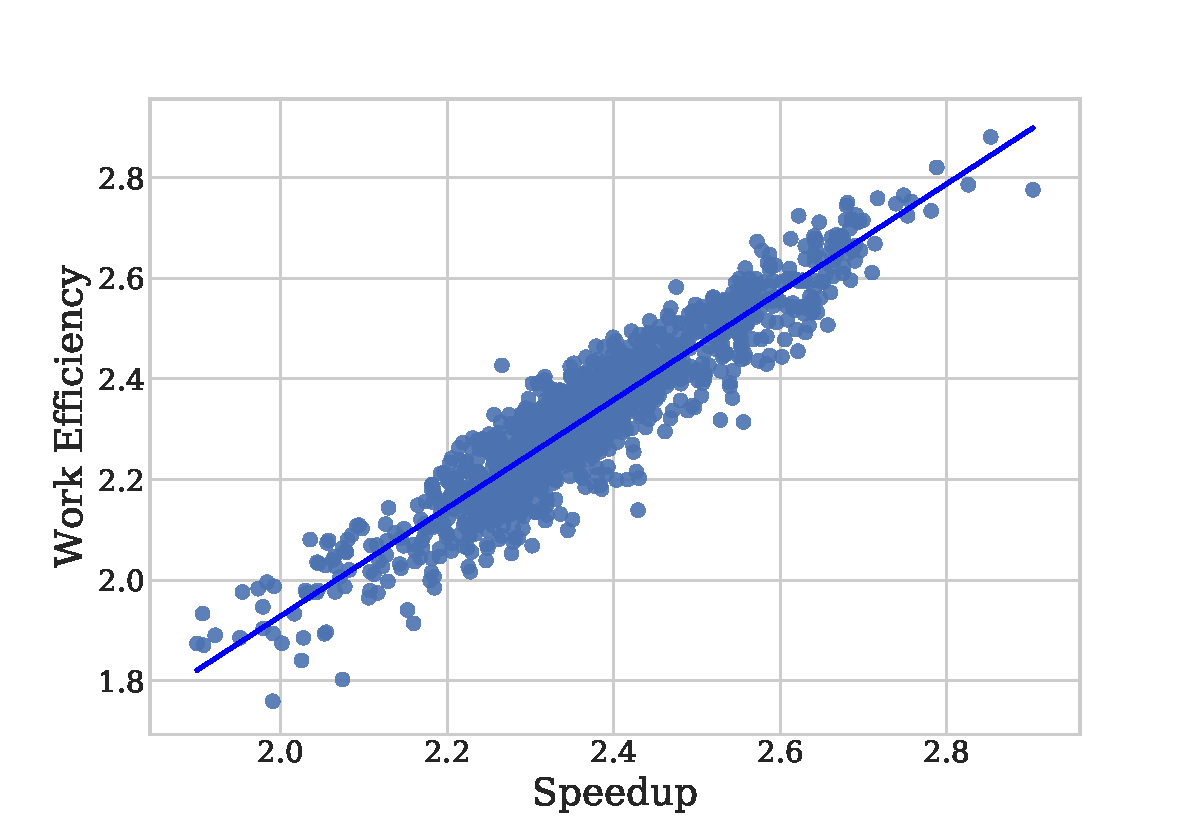
\includegraphics[width=0.5\textwidth]{figs/motivation-work-efficiency.pdf}
        \caption{Relationship between work efficiency vs speedup for 500 different binaries of \texttt{susan\_c}.
                Each point represents averages over a subset of all inputs.}
        \label{fig:motivation-work-efficiency}
    \end{figure}

